\chapter{半导体中载流子的统计分布}

\section{状态密度}

\subsection{状态密度}

半导体的\textbf{状态密度}$g(E)$定义为:
\begin{equation}
    g(E)=\frac{\mathrm{d}Z}{\mathrm{d}E}\label{eq:chap-3-state-density}
\end{equation}
其中$\mathrm{d}Z$为$\mathrm{d}E$能量区间下的量子态数。

通过1.2节的讨论,半导体中波矢$\bm k$的取值受到一定条件的限制。在线度$L$的半导体晶体中,$\bm k$的取值只能是
\begin{equation}
\left\{
\begin{aligned}
    k_x&=\frac{2\pi n_x}{L}\quad (n_x=0,\ \pm 1,\ \pm 2,\cdots)\\
    k_y&=\frac{2\pi n_y}{L}\quad (n_x=0,\ \pm 1,\ \pm 2,\cdots)\\
    k_z&=\frac{2\pi n_z}{L}\quad (n_x=0,\ \pm 1,\ \pm 2,\cdots)
\end{aligned}
\right.
\end{equation}
故$\bm k$空间的量子态密度为:
\begin{equation}
    2\times\left(\frac{2\pi}{L}\right)^3=\frac{2V}{8\pi^3}
\end{equation}
其中$V=L^3$为晶体体积。半导体的能带(导带)极值附近有:
\begin{equation}
    E(k)=E_c+\frac{\hslash^2k^2}{2m_n^*}
\end{equation}
故有:
\begin{align}
    &k=\frac{\left(2m_n^*\right)^\frac{1}{2}\left(E-E_c\right)^\frac{1}{2}}{\hslash}\label{eq:chap-3-energy-band-k(E)}\\
    &k\mathrm{d}k=\frac{m_n^*\mathrm{d}E}{\hslash^2}\label{eq:chap-3-energy-band-kdk(E)}
\end{align}

在$\bm k$空间中,以$|\bm k|$为半径作球面,即$E(k)$的等能面;再以$|\bm k+\mathrm{d}\bm k|$为半径作球面,即$E(k)+\mathrm{d}E$的等能面。$\mathrm{d}E$球壳体积$4\pi k^2\mathrm{d}k$,计算$\mathrm{d}E$球壳的量子态数$\mathrm{d}Z$:
\begin{equation}
    \mathrm{d}Z=\frac{2V}{8\pi^3}\times4\pi k^2\mathrm{d}k\label{eq:chap-3-fun-dZ(dk)}
\end{equation}
代入\autoref{eq:chap-3-energy-band-k(E)}和\autoref{eq:chap-3-energy-band-kdk(E)},得:
\begin{equation}
    \mathrm{d}Z=\frac{V}{2\pi^2}\frac{\left(2m_n^*\right)^\frac{3}{2}}{\hslash^3}\left(E-E_c\right)^\frac{1}{2}\mathrm{d}E
\end{equation}
由\autoref{eq:chap-3-state-density}得到导带底部附近状态密度:
\begin{equation}
    g_c(E)=\frac{\mathrm{d}Z}{\mathrm{d}E}=\frac{V}{2\pi^2}\frac{\left(2m_n^*\right)^\frac{3}{2}}{\hslash^3}\left(E-E_c\right)^\frac{1}{2}\label{eq:chap-3-cond-state-density-fun}
\end{equation}

\subsection{状态密度有效质量}

对于实际半导体(如Si、Ge),它在导带附近的等能面是旋转椭球面。取极值能量$E_c$,有:
\begin{equation}
    E(k)=E_c+\frac{\hslash^2}{2}\left[\frac{k_1^2+k_2^2}{m_t}+\frac{k_3^2}{m_l}\right]
\end{equation}
此时的状态密度
\begin{equation}
    g_c(E)=\frac{V}{2\pi^2}\frac{\left(2m_n^*\right)^\frac{3}{2}}{\hslash^3}(E-E_c)^\frac{1}{2}
\end{equation}
其中$m_n^*$为
\begin{equation}
    m_n^*=m_{dn}=s^\frac{2}{3}\left(m_lm_t^2\right)^\frac{1}{3}
\end{equation}
$m_{dn}$为\textbf{导带底状态密度有效质量}。对Si,$s=6$;对Ge,$s=4$。

\section{费米能级和载流子统计分布}

\subsection{费米分布函数}

对于能量为$E$的量子态,它被一个电子占据的概率$f(E)$为:
\begin{equation}
    f(E)=\frac{1}{1+\exp{\left(\frac{E-E_F}{k_0T}\right)}}
\end{equation}
$f(E)$称为\textbf{费米分布函数}。它描述\textbf{热平衡}下,电子在允许量子态上的分布情况。$k_0$是玻尔兹曼常数,$T$是热力学温度。$E_F$是\textbf{费米能级},统计物理证明,费米能级是系统的化学势:
\begin{equation}
    E_F=\mu=\left(\frac{\partial F}{\partial N}\right)_T
\end{equation}

\subsection{玻尔兹曼分布函数}

\vspace{1ex}$E-E_F\gg k_0T$时,由于$\D\exp{\frac{E-E_F}{k_0 T}}\gg 1$,有:
\begin{equation}
    1+\exp{\left(\frac{E-E_F}{k_0T}\right)}\approx\exp{\left(\frac{E-E_F}{k_0T}\right)}
\end{equation}
此时费米分布转化为玻尔兹曼分布:
\begin{equation}
    f_B(E)=\exp{\left(-\frac{E-E_F}{k_0T}\right)}=\exp{\left(\frac{E_F}{k_0T}\right)}\exp{\left(-\frac{E}{k_0T}\right)}
\end{equation}
\vspace{1ex}令$A=\D\exp{\left(\frac{E_F}{k_0T}\right)}$,则
\begin{equation}
    f_B(E)=A\exp{\left(-\frac{E}{k_0T}\right)}
    \label{eq:chap-3-electron-distribute-fun}
\end{equation}

$f(E)$是能量$E$的电子态被电子占据的概率,则$1-f(E)$是能量$E$的量子态不被电子占据的概率,即\textbf{空穴}占据的概率:
\begin{equation}
    1-f(E)=\frac{1}{1+\exp{\left(\frac{E_F-E}{k_0T}\right)}}
\end{equation}
\vspace{1ex}$E_F-E\gg k_0T$时,设$B=\exp{\left(-\frac{E_F}{k_0T}\right)}$,则:
\begin{equation}
    1-f(E)=B\exp{\left(\frac{E}{k_0T}\right)}
\end{equation}
上式即空穴的玻尔兹曼分布函数。

\subsection{导带中电子浓度和价带中空穴浓度}

非简并条件下,能量在$E\sim E+\mathrm{d}E$间的电子数$\mathrm{d}N$为:
\begin{equation}
    \mathrm{d}N=f_B(E)g_c(E)\mathrm{d}E
\end{equation}
代入\autoref{eq:chap-3-cond-state-density-fun}的$g_c(E)$和\autoref{eq:chap-3-electron-distribute-fun}的$f_B(E)$,得:
\begin{equation}
    \mathrm{d}N=\frac{V}{2\pi^2}\frac{\left(2m_n^*\right)^{\frac{3}{2}}}{\hslash^3}\exp{\left(-\frac{E-E_F}{k_0T}\right)}\left(E-E_c\right)^{\frac{1}{2}}\mathrm{d}E
\end{equation}
$E\sim E+\mathrm{d}E$间单位体积的电子数为:
\begin{equation}
    \mathrm{d}n=\frac{\mathrm{d}N}{V}=\frac{1}{2\pi^2}\frac{\left(2m_n^*\right)^{\frac{3}{2}}}{\hslash^3}\exp{\left(-\frac{E-E_F}{k_0T}\right)}\left(E-E_c\right)^{\frac{1}{2}}\mathrm{d}E\label{eq:chap-3-electron-number-in-dE-unit-volume}
\end{equation}
积分计算热平衡下非简并半导体的\textbf{导带电子浓度}$n_0$:
\begin{equation}
    n_0=\int_{E_c}^{E_c'}\frac{1}{2\pi^2}\frac{\left(2m_n^*\right)^{\frac{3}{2}}}{\hslash^3}\exp{\left(-\frac{E-E_F}{k_0T}\right)}\left(E-E_c\right)^{\frac{1}{2}}\mathrm{d}E
\end{equation}
\vspace{1ex}$E_c'$为导带顶能量,$E_c'\rightarrow +\infty$。取$\D x=\frac{E-E_c}{k_0T}$,利用积分公式
\begin{equation}
    \int_0^\infty x^\frac{1}{2}\mathrm{e}^{-x}\mathrm{d}x=\frac{\sqrt{\pi}}{2}
\end{equation}
求得导带电子浓度
\begin{equation}
    n_0=2\left(\frac{m_n^*k_0T}{2\pi\hslash^2}\right)^\frac{3}{2}\exp{\left(-\frac{E_c-E_F}{k_0T}\right)}
\end{equation}
令
\begin{equation}
    N_c=2\left(\frac{m_n^*k_0T}{2\pi\hslash^2}\right)^\frac{3}{2}=2\frac{\left(2\pi m_n^*k_0T\right)^\frac{3}{2}}{h^{3}}
\end{equation}
得
\begin{equation}
    n_0=N_c\exp{\left(-\frac{E_c-E_F}{k_0T}\right)}\label{eq:chap-3-cond-electron-concentration}
\end{equation}
\vspace{1ex}$N_c$为\textbf{导带有效状态密度}。显然有$N_c\propto\D T^\frac{3}{2}$。$\D \exp{\left(-\frac{E_c-E_F}{k_0T}\right)}$是电子占据导带底$E_c$的概率。

同理,\textbf{价带空穴浓度}$p_0$为:
\begin{align}
    p_0&=\int_{E_v'}^{E_v}\left[1-f(E)\right]\frac{g_v(E)}{V}\mathrm{d}E\\
    &=\frac{1}{2\pi^2}\frac{(2m_p^*)^\frac{3}{2}}{\hslash^3}\int_{E_v'}^{E_v}\exp{\left(\frac{E-E_F}{k_0T}\right)}\left(E-E_F\right)^\frac{1}{2}\mathrm{d}E
\end{align}
$E_v'\rightarrow -\infty$,利用积分公式,得:
\begin{equation}
    p_0=2\left(\frac{m_p^* k_0T}{2\pi\hslash^2}\right)^\frac{3}{2}\exp{\left(\frac{E_v-E_F}{k_0T}\right)}
\end{equation}
令\begin{equation}
    N_v=2\left(\frac{m_p^* k_0T}{2\pi\hslash^2}\right)^\frac{3}{2}=2\frac{\left(2\pi m_p^*k_0T\right)^\frac{3}{2}}{h^3}
\end{equation}
得
\begin{equation}
    p_0=N_v\exp{\left(\frac{E_v-E_F}{k_0T}\right)}\label{eq:chap-3-val-hole-concentration}
\end{equation}
$N_v$为\textbf{价带有效状态密度}。显然$\D N_v\propto T^\frac{3}{2}$,$\D \exp{\left(\frac{E_v-E_F}{k_0T}\right)}$是空穴占据价带顶$E_v$的概率。

\subsection{载流子浓度乘积\texorpdfstring{$n_0p_0$}{n₀p₀}}

将\autoref{eq:chap-3-cond-electron-concentration}和\autoref{eq:chap-3-val-hole-concentration}相乘,得到\textbf{载流子浓度乘积}:
\begin{equation}
    n_0p_0=N_cN_v\exp{\left(-\frac{E_c-E_v}{k_0T}\right)}=N_cN_v\exp{\left(-\frac{E_g}{k_0T}\right)}\label{eq:chap-3-charge-carrier-concentration-production}
\end{equation}
$E_g$为禁带宽度。代入$N_c$和$N_v$表达式,得:
\begin{align}
    n_0p_0&=4\left(\frac{k_0}{2\pi\hslash^2}\right)^3\left(m_n^*m_p^*\right)^\frac{3}{2}T^3\exp{\left(-\frac{E_g}{k_0T}\right)}\\
    &=2.33\times 10^{31}\left(\frac{m_n^*m_p^*}{m_0^2}\right)^\frac{3}{2}T^3\exp{\left(-\frac{E_g}{k_0T}\right)}
\end{align}

\section{本征半导体的载流子浓度}

\textbf{本征载流子}即没有杂质和缺陷的半导体。$T=0\ \mathrm{K}$时价带中全部量子态被电子占据,导带量子态全空。$T>0\ \mathrm{K}$时,电子从价带激发到导带,同时在价带中产生空穴,即\textbf{本征激发}。

本征半导体中,电子和空穴成对出现,电子浓度等于空穴浓度:
\begin{equation}
    n_0=p_0\label{eq:chap-3-intrinsic-excitation}
\end{equation}
即本征激发的\textbf{电中性条件}。

将\autoref{eq:chap-3-cond-electron-concentration}和\autoref{eq:chap-3-val-hole-concentration}代入上式,求得本征半导体的费米能级$E_F$,用$E_i$表示:
\begin{equation}
    N_c\exp{\left(-\frac{E_c-E_F}{k_0T}\right)}=N_v\exp{\left(-\frac{E_F-E_v}{k_0T}\right)}
\end{equation}
取对数:
\begin{equation}
    E_i=E_F=\frac{E_c+E_v}{2}+\frac{k_0T}{2}\ln{\frac{N_v}{N_c}}
\end{equation}
代入$N_c$和$N_v$表达式:
\begin{equation}
    E_i=E_F=\frac{E_c+E_v}{2}+\frac{3k_0T}{4}\ln{\frac{m_p^*}{m_n^*}}\label{eq:chap-3-intrinsic-fermi-energy}
\end{equation}
将\autoref{eq:chap-3-intrinsic-fermi-energy}反代入\autoref{eq:chap-3-cond-electron-concentration}和\autoref{eq:chap-3-val-hole-concentration},得到本征载流子浓度$n_i$:
\begin{equation}
    n_i=n_0=p_0=\left(N_cN_v\right)^\frac{1}{2}\exp{\left(-\frac{E_g}{2k_0T}\right)}\label{eq:chap-3-intrinsic-charge-carrier-concentration}
\end{equation}
比较\autoref{eq:chap-3-charge-carrier-concentration-production}和\autoref{eq:chap-3-intrinsic-charge-carrier-concentration}得:
\begin{equation}
    n_0p_0=n_i^2\label{eq:chap-3-intinsic-charge-carrier-concentration-equation}
\end{equation}
上式表明:一定温度下,任何非简并半导体热平衡载流子浓度乘积$n_0p_0$等于该温度下本征载流子浓度$n_i$的平方。

代入$N_c$和$N_v$表达式:
\begin{align}
    n_i&=\left[\frac{2\left(2\pi k_0T\right)^\frac{3}{2}\left(m_p^*m_n^*\right)^\frac{3}{4}}{h^3}\right]\exp{\left(-\frac{E_g}{2k_0T}\right)}\\
    &=4.82\times 10^{15}\times\left(\frac{m_p^*m_n^*}{m_0^*}\right)^\frac{3}{4}T^\frac{3}{2}\exp{\left(-\frac{E_g}{2k_0T}\right)}
\end{align}

\section{杂质半导体的载流子浓度}

\subsection{杂质能级上的电子和空穴}

含有杂质的半导体中,杂质部分电离。电子占据杂质能级的概率不能用费米分布函数决定,因为能带中的能级能容纳两个自旋相反的电子,而杂质能级要么只能被一个具有任一自旋方向的电子占据,要么完全不接受电子。记$E_D$为施主能级,电子占据施主能级的概率表达式
\begin{equation}
    f_D(E)=\frac{1}{\D 1+\frac{1}{g_D}\exp{\left(\frac{E_D-E_F}{k_0T}\right)}}
\end{equation}
记$E_A$为受主能级,空穴占据受主能级概率
\begin{equation}
    f_A(E)=\frac{1}{\D 1+\frac{1}{g_A}\exp{\left(\frac{E_F-E_A}{k_0T}\right)}}
\end{equation}
$g_D$为\textbf{施主能级基态简并度},$g_A$为\textbf{受主能级基态简并度},通常称为\textbf{简并因子}。对于Ge、Si、GaAs等材料,$g_D=2,\ g_A=4$。

记$N_D$为施主浓度,$N_A$为受主浓度。则$N_D$和$N_A$记为杂质的量子态密度。电子和空穴占据杂质能级的概率分别为$f_D(E)$和$f_A(E)$,因此:\vspace{1ex} \\
(1) 施主能级上的电子浓度$n_D$为:
\begin{equation}
    n_D=N_Df_D(E)=\frac{N_D}{\D 1+\frac{1}{g_D}\exp{\left(\frac{E_D-E_F}{k_0T}\right)}}\label{eq:chap-3-donor-electron-concentration}
\end{equation}
这也是没有电离的施主浓度。\vspace{1ex} \\
(2) 受主能级上的空穴浓度$p_A$为:
\begin{equation}
    p_A=N_Af_A(E)=\frac{N_A}{\D 1+\frac{1}{g_A}\exp{\left(\frac{E_F-E_A}{k_0T}\right)}}\label{eq:chap-3-acceptor-hole-concentration}
\end{equation}
这也是没有电离的受主浓度。\vspace{1ex} \\
(3) 电离施主浓度$n_D^+$为:
\begin{equation}
    n_D^+=N_D-n_D=N_D\left[1-f_D(E)\right]=\frac{N_D}{\D 1+g_D\exp{\left(-\frac{E_D-E_F}{k_0T}\right)}}\label{eq:chap-3-ionized-donor-concentration}
\end{equation}
(4) 电离受主杂质浓度$p_A^+$为:
\begin{equation}
    p_A^-=N_A-p_A=N_A\left[1-f_A(E)\right]=\frac{N_A}{\D 1+g_A\exp{\left(-\frac{E_F-E_A}{k_0T}\right)}}\label{eq:chap-3-ionized-acceptor-concentration}
\end{equation}

\subsection{n型半导体的载流子浓度}

n型半导体单位体积的负电荷数,即导带中电子浓度$n_0$,等于单位体积的正电荷数,即价带中空穴浓度$p_0$与电离施主浓度$n_D^+$之和。即电中性条件:
\begin{equation}
    n_0=n_D^++p_0\label{eq:chap-3-n-type-semi-neutrality}
\end{equation}

取$g_D=2$,将\autoref{eq:chap-3-cond-electron-concentration}、\autoref{eq:chap-3-val-hole-concentration}和\autoref{eq:chap-3-ionized-donor-concentration}代入上式:
\begin{equation}
    N_c\exp{\left(-\frac{E_c-E_F}{k_0T}\right)}=N_v\exp{\left(-\frac{E_F-E_v}{k_0T}\right)}+\frac{N_D}{\D 1+2\exp{\left(-\frac{E_D-E_F}{k_0T}\right)}}\label{eq:chap-3-n-type-neutral-equation}
\end{equation}
上式直接求取$E_F$是困难的。我们分析在不同温度情况下的情况。\vspace{1ex} \\
\textbf{1. 低温弱电离区}\vspace{1ex}

温度很低时,大部分施主杂质不发生电离,少部分施主杂质发生电离,少量电子进入导带,称为\textbf{弱电离}。从价带跃迁到导带的电子则更少,可以忽略不计。故$p_0=0,\ n_0=n_D^+$,即:
\begin{equation}
    N_c\exp{\left(-\frac{E_c-E_F}{k_0T}\right)}=\frac{N_D}{\D 1+2\exp{\left(-\frac{E_D-E_F}{k_0T}\right)}}
\end{equation}
\vspace{1ex}由于$n_D^+\ll N_D$,所以$\D \exp{\left(-\frac{E_D-E_F}{k_0T}\right)}\gg 1$,上式继续简化为:
\begin{equation}
    N_c\exp{\left(-\frac{E_c-E_F}{k_0T}\right)}=\frac{1}{2}N_D\exp{\left(\frac{E_D-E_F}{k_0T}\right)}
\end{equation}
取对数化简:
\begin{equation}
    E_F=\frac{E_c+E_D}{2}+\left(\frac{k_0T}{2}\right)\ln{\left(\frac{N_D}{2N_c}\right)}\label{eq:chap-3-low-T-weak-ionize-fermi-energy}
\end{equation}
上式即低温弱电离区费米能级表达式。

\vspace{1ex}由于$N_c\propto T^\frac{3}{2}$,低温极限$T\rightarrow 0\ \mathrm{K}$时,$\D \lim_{T\rightarrow 0 \mathrm{K}}\left(T\ln{T}\right)=0$,故
\begin{equation}
    \lim_{T\rightarrow 0\mathrm{K}}E_F=\frac{E_c+E_D}{2}
\end{equation}
即低温极限下,费米能级在导带底和施主能级中线处。\vspace{1ex} \\
\textbf{2. 中间电离区}\vspace{1ex}

\vspace{1ex}温度升高,在$2N_c>N_D$后,\autoref{eq:chap-3-low-T-weak-ionize-fermi-energy}第二项变为负值,$E_F$降至$\D \frac{E_c+E_D}{2}$以下。温度继续升高,$\D \exp{\left(\frac{E_F-E_D}{k_0T}\right)}=1$时,$E_F=E_D$,施主杂质$\D \frac{1}{3}$电离。\vspace{1ex} \\
\textbf{3. 强电离区}\vspace{1ex}

\vspace{1ex}温度升高到大部分杂质均电离,称为\textbf{强电离区}。此时$n_D^+\approx N_D$,有$\D \exp{\left(\frac{E_F-E_D}{k_0T}\right)}\ll 1$或$E_D-E_F\gg k_0T$。费米能级$E_F$在施主能级$E_D$之下。\autoref{eq:chap-3-n-type-neutral-equation}简化为:
\begin{equation}
    N_c\exp{\left(-\frac{E_c-E_F}{k_0T}\right)}=N_D\label{eq:chap-3-n-type-stronge-ionize-equation}
\end{equation}
解得费米能级$E_F$为:
\begin{equation}
    E_F=E_c+k_0T\ln{\left(\frac{N_D}{N_c}\right)}\label{eq:chap-3-n-type-stronge-ionize-fermi-energy}
\end{equation}

施主杂质全部电离时,电子浓度$n_0$为:
\begin{equation}
    n_0=N_D
\end{equation}
载流子浓度与温度无关。载流子浓度等于杂质浓度的温度范围称为\textbf{饱和区}。

当$(E_D-E_F)\gg k_0T$时,施主能级上的电子浓度$n_D$表达式\autoref{eq:chap-3-donor-electron-concentration}简化为:
\begin{equation}
    n_D\approx 2N_D\exp{\left(-\frac{E_D-E_F}{k_0T}\right)}
\end{equation}
代入\autoref{eq:chap-3-n-type-stronge-ionize-equation},得:
\begin{equation}
    n_D\approx 2N_D\left(\frac{N_D}{N_c}\right)\exp{\left(\frac{E_c-E_D}{k_0T}\right)}=2N_D\left(\frac{N_D}{N_c}\right)\exp{\left(\frac{\Delta E_D}{k_0T}\right)}
\end{equation}
令
\begin{equation}
    D_-=\left(\frac{2N_D}{N_c}\right)\exp{\left(\frac{\Delta E_D}{k_0T}\right)}
\end{equation}
得到:
\begin{equation}
    n_D\approx D_-N_D
\end{equation}
由于$N_D$是施主杂质浓度,$n_D$是未电离施主浓度,因此$D_-$的物理意义是\textbf{未电离施主占施主杂质的百分比}。\vspace{1ex}\\
\textbf{4. 过渡区}\vspace{1ex}

升高温度,使半导体处于饱和区和本征激发区(本征激发产生的本征载流子远多于杂质产生的载流子)之间,称为\textbf{过渡区}。此时导带中的电子一部分来源于全部电离的杂质,另一部分由本征激发提供。电中性条件为:
\begin{equation}
    n_0=N_D+p_0\label{eq:chap-3-transition-neutral-condition}
\end{equation}
其中$n_0$为导带电子浓度,$p_0$为价带中的空穴浓度,$N_D$为全部电离的施主杂质浓度。

本征激发时,有:
\begin{align}
    n_0=p_0=n_i \\
    E_F=E_i
\end{align}
得到
\begin{align}
    &n_i=N_c\exp{\left(-\frac{E_c-E_i}{k_0T}\right)}\\
    \Longrightarrow&N_c=n_i\exp{\left(\frac{E_c-E_i}{k_0T}\right)}
\end{align}
代入\autoref{eq:chap-3-cond-electron-concentration},得:
\begin{equation}
    n_0=n_i\exp{\left(-\frac{E_i-E_F}{k_0T}\right)}
\end{equation}
同理有:
\begin{equation}
    p_0=n_i\exp{\left(\frac{E_i-E_F}{k_0T}\right)}
\end{equation}
代入\autoref{eq:chap-3-transition-neutral-condition},得:
\begin{equation}
    N_D=n_0-p_0=n_i\left[\exp{\left(\frac{E_F-E_i}{k_0T}\right)}-\exp{\left(-\frac{E_F-E_i}{k_0 T}\right)}\right]=2n_i\sinh{\left(\frac{E_F-E_i}{k_0T}\right)}
\end{equation}
解得
\begin{equation}
    E_F=E_i+k_0T\mathop{\mathrm{asinh}{\left(\frac{N_D}{2n_i}\right)}}
\end{equation}

计算过渡区载流子浓度$n_0$和$p_0$,可以联立方程\autoref{eq:chap-3-intinsic-charge-carrier-concentration-equation}和\autoref{eq:chap-3-transition-neutral-condition}:
\begin{equation}
    \left\{
    \begin{aligned}
        &p_0=n_0-N_D\\
        &n_0p_0=n_i^2
    \end{aligned}
    \right.
\end{equation}
消去$p_0$:
\begin{equation}
    n_0^2-N_Dn_0-n_i^2=0
\end{equation}
取方程正根,解得:
\begin{equation}
    n_0=\frac{N_D+\sqrt{N_D^2+4n_i^2}}{2}=\frac{N_D}{2}\left[1+\sqrt{1+\frac{4n_i^2}{N_D^2}}\right]
\end{equation}
于是
\begin{equation}
    p_0=\frac{n_i^2}{n_0}=\left(\frac{2n_i^2}{N_D}\right)\left[1+\sqrt{1+\frac{4n_i^2}{N_D^2}}\right]^{-1}
\end{equation}
\vspace{1ex}当$N_D\gg n_i$时,$\D \frac{4n_i^2}{N_D^2}\ll 1$,将因子$\D \sqrt{1+\frac{4n_i^2}{N_D^2}}$级数展开到一次项:
\begin{equation}
    \left(1+\frac{4n_i^2}{N_D^2}\right)^\frac{1}{2}=1+\frac{1}{2}\frac{4n_i^2}{N_D^2}+\mathcal{O}\left[\left(\frac{4n_i^2}{N_D^2}\right)^2\right]
\end{equation}
代入,得:
\begin{align}
    &n_0=N_D+\frac{n_i^2}{N_D}\\
    &p_0=n_0-N_D\frac{n_i^2}{N_D}
\end{align}
当$N_D\ll n_i$时
\begin{align}
    n_0&=\frac{N_D}{2}\left[1+\sqrt{1+\frac{4n_i^2}{N_D^2}}\right]\\
    &=\frac{N_D}{2}+\left(\frac{N_D^2}{4}+n_i^2\right)^\frac{1}{2}\\
    &=\frac{N_D}{2}+n_i\left(1+\frac{N_D^2}{4n_i^2}\right)^\frac{1}{2}
\end{align}
\vspace{1ex}此时由于$N_D\ll n_i$,有$\D \frac{N_D^2}{4n_i^2}\ll 1$,所以:
\begin{align}
    &n_0=\frac{N_D}{2}+n_i\\
    &p_0=-\frac{N_D}{2}+n_i
\end{align}
$n_0$和$p_0$数量相近,均趋近于$n_i$。\vspace{1ex}\\
\textbf{5. 高温本征激发区}\vspace{1ex}

此时本征激发产生的本征载流子远多于杂质产生的载流子,即$n_0\gg N_D,\ p_0\gg N_D$。此时的电中性条件是:
\begin{equation}
    n_0=p_0
\end{equation}
与未掺杂的本征载流子情况一致。\vspace{1ex}\\
\textbf{6. p型半导体的载流子浓度}\vspace{1ex}

受主浓度$N_A$的p型半导体,取$g_A=4$,与上面n型半导体的讨论相似,可以得到以下结论:
\begin{enumerate}
    \item 低温弱电离区:
    \begin{align}
        &E_F=\frac{E_v+E_A}{2}-\left(\frac{k_0T}{2}\right)\ln{\left(\frac{N_A}{4N_v}\right)}\\
        &p_0=\left(\frac{N_AN_v}{4}\right)^\frac{1}{2}\exp{\left(-\frac{\Delta E_A}{2k_0T}\right)}
    \end{align}
    \item 强电离区:
    \begin{align}
        &E_F=E_v-k_0T\ln{\left(\frac{N_A}{N_v}\right)}\\
        &p_0=N_A\\
        &p_A=D_+N_A\\
        &D_+=\left(\frac{4N_A}{N_v}\right)\exp{\left(\frac{\Delta E_A}{k_0T}\right)}
    \end{align}
    $D_+$是未电离受主杂质百分数。
    \item 过渡区:
    \begin{align}
        &E_F=E_i-k_0T\mathop{\mathrm{asinh}{\left(\frac{N_A}{2n_i}\right)}}\\
        &p_0=\left(\frac{N_A}{2}\right)\left[1+\sqrt{1+\frac{4n_i^2}{N_A^2}}\right]\\
        &n_0=\left(\frac{2n_i^2}{N_A}\right)\left[1+\sqrt{1+\frac{4n_i^2}{N_A^2}}\right]^{-1}
    \end{align}
\end{enumerate}
\textbf{7. 少数载流子浓度}\vspace{1ex}

n型半导体中的电子和p型半导体中的空穴称为\textbf{多数载流子}(\textbf{多子}),n型半导体中的空穴和p型半导体中的电子称为\textbf{少数载流子}(\textbf{少子})。
\begin{enumerate}[(1)]
    \item n型半导体:记$n_{n0}$为\textbf{热平衡下n型半导体电子(多子)浓度},$p_{n0}$为\textbf{热平衡下n型半导体空穴(少子)浓度}。多子浓度$n_{n0}=N_D$。由$n_{n0}p_{n0}=n_i^2$关系,得到少子浓度$p_{n0}$:
    \begin{equation}
        p_{n0}=\frac{n_i^2}{N_D}
    \end{equation}
    \item p型半导体:记$p_{p0}$为\textbf{热平衡下p型半导体空穴(多子)浓度},$n_{p0}$为\textbf{热平衡下p型半导体电子(少子)浓度}。多子浓度$p_{p0}=N_A$,由$n_{p0}p_{p0}=n_i^2$关系,得到少子浓度$n_{p0}$:
    \begin{equation}
        n_{p0}=\frac{n_i^2}{N_A}
    \end{equation}
\end{enumerate}

\section{一般情况下的载流子分布}

单位体积内有$n$个电子,$p$个空穴,电离施主浓度为$n_D^+$,电离受主浓度为$p_A^-$,带电均为$q$,净空间电荷密度$\rho$为:
\begin{equation}
    \rho=q\left(p+n_D^+-n-p_A^-\right)
\end{equation}
热平衡时:
\begin{equation}
    \rho_0=q\left(p_0+n_D^+-n_0-p_A^-\right)
\end{equation}
半导体电中性,热平衡下有条件$\rho_0=0$,得:
\begin{equation}
    p_0+n_D^+=n_0+p_A^-\label{eq:chap-3-1-donor-1-receiver-neutral-charge-condition}
\end{equation}
上式即含有一种受主杂质和一种受主杂质的半导体的电中性条件。半导体若存在若干受主杂质和施主杂质,电中性条件改为:
\begin{equation}
    p_0+\sum_{j}n_{Dj}^+=n_0+\sum_{i}p_{Ai}^-
\end{equation}
\vspace{1ex}$\D \sum_{j}n_{Dj}^+$和$\D \sum_{i}p_{Ai}^-$是对诸电离施主和受主杂质的求和。

由于$n_D^+=N_D-n_D,\ p_A^-=N_A-p_A$,代入电中性条件\autoref{eq:chap-3-1-donor-1-receiver-neutral-charge-condition},得:
\begin{equation}
    p_0+N_D+p_A=n_0+N_A+n_D\label{eq:chap-3-1-donor-1-receiver-neutral-charge-condition-expand}
\end{equation}
将导带电子浓度$n_0$表达式\autoref{eq:chap-3-cond-electron-concentration},价带空穴浓度$p_0$表达式\autoref{eq:chap-3-val-hole-concentration},施主能级上电子浓度(未电离施主杂质)\autoref{eq:chap-3-donor-electron-concentration},受主能级上空穴浓度(未电离受主浓度)\autoref{eq:chap-3-acceptor-hole-concentration}代入上式\autoref{eq:chap-3-1-donor-1-receiver-neutral-charge-condition-expand},并取$g_D=2,\ g_A=4$,得:
\begin{equation}
\begin{aligned}
    &N_D+N_v\exp{\left(\frac{E_v-E_F}{k_0T}\right)}+\frac{N_A}{\D 1+\frac{1}{4}\exp{\left(-\frac{E_A-E_F}{k_0T}\right)}}\\
    =&N_A+N_c\exp{\left(-\frac{E_c-E_F}{k_0T}\right)}+\frac{N_D}{\D 1+\frac{1}{2}\exp{\left(\frac{E_D-E_F}{k_0T}\right)}}
\end{aligned}
\end{equation}
对于确定的半导体,$N_A,\ N_D,\ E_c,\ E_v,\ E_A,\ E_D$已知,一定温度下$N_c,\ N_v$也可计算得到,即可通过这一关系确定$E_F$。

\section{简并半导体}

\subsection{简并半导体的载流子浓度}

对于前几节的讨论,我们认为费米能级$E_F$在禁带中,且$E_c-E_F\gg k_0T$或$E_F-E_v\gg k_0T$。此时导带电子和价带空穴服从玻尔兹曼分布,浓度表达式:
\begin{align}
    &n_0=N_c\exp{\left(-\frac{E_c-E_F}{k_0T}\right)}\\
    &p_0=N_v\exp{\left(-\frac{E_F-E_v}{k_0T}\right)}
\end{align}
但当$E_F$接近或进入导带时,$E_c-E_F\gg k_0T$的条件不满足,此时电子浓度需用费米分布函数计算。此时简并半导体电子浓度$n_0$为:
\begin{equation}
    n_0=\int_{E_c}^\infty\frac{g_c(E)f(E)}{V}=\frac{\left(2m_n^*\right)^\frac{3}{2}}{2\pi^2\hslash^3}\int_{E_c}^\infty\frac{\left(E-E_c\right)^\frac{1}{2}}{\D 1+\exp{\left(\frac{E-E_F}{k_0T}\right)}}\mathrm{d}E
\end{equation}
\vspace{1ex}我们仍设$\D N_c=2\left(\frac{m_n^*k_0T}{2\pi\hslash}\right)^\frac{3}{2}=2\frac{\left(2\pi m_n^*k_0T\right)^\frac{3}{2}}{h^3}$,并令
\begin{equation}
    x=\frac{E-E_c}{k_0T},\quad \xi=\frac{E_F-E_c}{k_0T}
\end{equation}
则有:
\begin{equation}
    n_0=N_c\frac{2}{\sqrt{\pi}}\int_0^\infty\frac{x^\frac{1}{2}}{1+\mathrm{e}^{x-\xi}}\mathrm{d}x
\end{equation}
其中积分
\begin{equation}
    \int_0^\infty\frac{x^\frac{1}{2}}{1+\mathrm{e}^{x-\xi}}\mathrm{d}x=F_\frac{1}{2}(\xi)=F_\frac{1}{2}\left(\frac{E_F-E_c}{k_0T}\right)
\end{equation}
称为\textbf{费米积分}。$n_0$可写为:
\begin{equation}
    n_0=N_c\frac{2}{\sqrt{\pi}}F_\frac{1}{2}(\xi)=N_c\frac{2}{\sqrt{\pi}}F_\frac{1}{2}\left(\frac{E_F-E_c}{k_0T}\right)
\end{equation}

当$E_F$接近或进入价带时,同理可得简并半导体价带空穴浓度为:
\begin{equation}
    p_0=N_v\frac{2}{\sqrt{\pi}}F_\frac{1}{2}\left(\frac{E_v-E_F}{k_0T}\right)
\end{equation}

\subsection{简并化条件}

经典统计中$\D \frac{n_0}{N_c}$与$\D \frac{E_F-E_c}{k_0}$关系:
\begin{equation}
    \frac{n_0}{N_c}=\exp{\left(\frac{E_F-E_c}{k_0T}\right)}
\end{equation}
在费米统计中,则是:
\begin{equation}
    \frac{n_0}{N_c}=\frac{2}{\sqrt{\pi}}F_\frac{1}{2}\left(\frac{E_F-E_c}{k_0T}\right)
\end{equation}
取对数坐标系,\autoref{fig:feimi-classical}可以看出费米统计与经典统计曲线的差别。
\begin{figure}
    \centering
    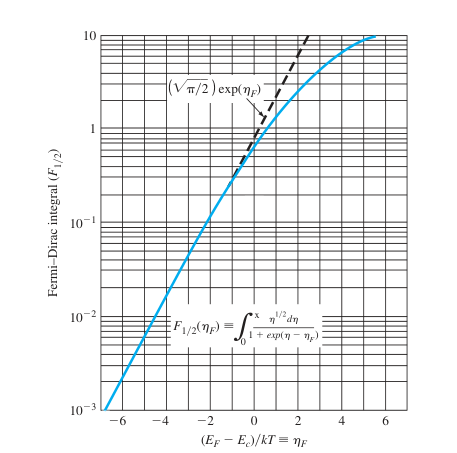
\includegraphics[width=0.8\linewidth]{feimi.png}
    \caption{费米统计与经典统计比较}
    \label{fig:feimi-classical}
\end{figure}
我们将$E_F$与$E_c$的相对位置作为区分简并与非简并的标准:
\begin{equation}
\left\{
\begin{aligned}
    &E_c-E_F>2k_0T \quad\text{非简并}\\
    &0<E_c-E_F\leq 2k_0T \quad\text{弱简并}\\
    &E_c-E_F\leq 0 \quad \text{简并}
\end{aligned}
\right.
\end{equation}



